\documentclass[a4paper]{article}

\usepackage[T1]{fontenc}
\usepackage[utf8]{inputenc}

\usepackage{mathptmx}

\usepackage{subcaption}
\usepackage[shortlabels]{enumitem}
\usepackage{amsmath,amssymb}
\usepackage{amsthm}
\usepackage{bbm}
\usepackage{graphicx}
\usepackage[colorlinks=true,naturalnames=true,plainpages=false,pdfpagelabels=true]{hyperref}
\usepackage[parfill]{parskip}

\usepackage{pst-node}
\usepackage{tikz-cd}

\usepackage{tikz}
\usetikzlibrary{patterns,decorations.pathmorphing,positioning}

\usepackage[framemethod=TikZ]{mdframed}

\tikzstyle{titlered} =
    [draw=black, thick, fill=white,%
        text=black, rectangle,
        right, minimum height=.7cm]

\newcounter{exercise}

\renewcommand*\theexercise{Exercise~\arabic{exercise}}

\makeatletter
\mdfdefinestyle{exercisestyle}{%
    outerlinewidth=1em,%
    outerlinecolor=white,%
    leftmargin=-1em,%
    rightmargin=-1em,%
    middlelinewidth=1.2pt,%
    roundcorner=5pt,%
    linecolor=black,%
    backgroundcolor=blue!5,
    innertopmargin=1.2\baselineskip,
    skipabove={\dimexpr0.5\baselineskip+\topskip\relax},
    skipbelow={-1em},
    needspace=3\baselineskip,
    frametitlefont=\sffamily\bfseries,
    settings={\global\stepcounter{exercise}},
    singleextra={%
        \node[titlered,xshift=1cm] at (P-|O) %
            {~\mdf@frametitlefont{\theexercise}~};},%
    firstextra={%
            \node[titlered,xshift=1cm] at (P-|O) %
                    {~\mdf@frametitlefont{\theexercise}~};},
}
\makeatother

\newenvironment{MyExercise}%
{\begin{mdframed}[style=exercisestyle]}{\end{mdframed}}

\theoremstyle{definition}
\newtheorem{definition}{Definition}

\theoremstyle{definition}
\newtheorem{question}{Question}

\theoremstyle{definition}
\newtheorem{example}{Example}

\theoremstyle{theorem}
\newtheorem{theorem}{Theorem}

\theoremstyle{theorem}
\newtheorem{lemma}{Lemma}

\theoremstyle{theorem}
\newtheorem{proposition}{Proposition}

\newtheorem*{idea}{Proof Idea}

\title{University of Vienna\\ Faculty of Physics\\ \vspace{1.25cm}
Notes on\\ Noncommutative Geometry and Particle Phyiscs}
\author{Milutin Popovic \\ Supervisor: Dr. Lisa
Glaser}
\date{Week 7: 23.04 - 27.04}

\begin{document}

    \maketitle
    \tableofcontents
    \newpage
\section{Classification of Finite Real Spectral Triples}

Here we classify finite real spectral triples modulo unitary equivalence with
\textit{Krajewski Diagrams}. We extend $\Lambda$-decorated graphs to the case of
real spectral triples (grading and real structure).

\textbf{The Algebra:}Like before:
\begin{align}
    A\simeq \bigoplus_{i=1}^N M_{n_i}(\mathbb{C}) \;\;\;\;\;\;\; \text{with} \;\;\; \hat{A} = \{\textbf{n}_1, \dots, \textbf{n}_N\}
\end{align}
Where $\textbf{n}_i$ are irreducible representation of $A$ on
$\mathbb{C}^{n_i}$

\textbf{The Hilbertspace:}Faithful irreducible representation on $A$ are the
direct sum of $\mathbb{C}^{n_i}$'s, which act on $A$ by left block-diagonal
matrix multiplication.
\begin{align}
    \bigoplus_{i=1}^N \mathbb{C}^{n_i}
\end{align}
Furthermore we need a representation of $A^\circ$ on $H$ that commutes with
$A$. That is
\begin{align}
    A^\circ \simeq &\bigoplus_{i=1}^N M_{n_i}(\mathbb{C})^\circ \\
        \text{with} \;\;\; &\hat{A}^\circ = \{\textbf{n}_1^\circ, \dots,
    \textbf{n}_N^\circ\} \\
    \text{and} \;\;\;  &\bigoplus_{i=1}^N \mathbb{C}^{n_i\circ}
\end{align}
And we need the multiplicity space $V_{ij}$ of $\mathbb{C}^{n_i} \otimes
\mathbb{C}^{n_j\circ}$.
Thus making the Hilbertspace:
\begin{align}
    H=\bigoplus_{i,j=1}^N \mathbb{C}^{n_i} \otimes \mathbb{C}^{n_j\circ}
    \otimes V_{ij}
\end{align}
\begin{itemize}
    \item $\textbf{n}_i$, $\textbf{n}_j^\circ$ form a grid
    \item if there is a node at $(\textbf{n}_i$, $\textbf{n}_j^\circ)$ then
            $\mathbb{C}^{n_i} \otimes \mathbb{C}^{n_j\circ}$ is nonzero in $H$.
    \item multiplicity implies multiple nodes
\end{itemize}

\begin{example}
    $A = \mathbb{C} \oplus M_2 (\mathbb{C})$, two options of the Hilbertspace.
    \begin{figure}[h!] \centering
    \begin{tikzpicture}[
        dot/.style = {draw, circle, inner sep=0.06cm},
        no/.style = {},
        ]
        \node[no](a) at (0,0) [label=left:$\textbf{1}^\circ$] {};
        \node[no](b) at (0, -1) [label=left:$\textbf{2}^\circ$] {};
        \node[no](c) at (1, 0.5) [label=above:$\textbf{1}$] {};
        \node[no](d) at (2, 0.5) [label=above:$\textbf{2}$] {};
        \node[dot](d0) at (1,0) [] {};
        \node[dot](d0) at (2,-1) [] {};

        \node[no](a1) at (6,0) [label=left:$\textbf{1}^\circ$] {};
        \node[no](b2) at (6, -1) [label=left:$\textbf{2}^\circ$] {};
        \node[no](c2) at (7, 0.5) [label=above:$\textbf{1}$] {};
        \node[no](d2) at (8, 0.5) [label=above:$\textbf{2}$] {};
        \node[dot](d0) at (7,0) [] {};
        \node[dot](d0) at (8,0) [] {};


        \end{tikzpicture}
    \end{figure}

The first diagram corresponds to $H_1 = \mathbb{C} \oplus M_2(\mathbb{C})$,
to the second $H_2 = \mathbb{C} \oplus \mathbb{C}^2$.
\end{example}

\begin{MyExercise}
    \textbf{Let $J$ be an anti-unitary operator on a finite-dimensional Hilbert space.
    Show that $J^2$ is an unitary operator
    } \newline

    Straight forward, say $J:\; H \rightarrow H$, then let $\xi_1, \xi_2 \in
    H$:

    \centering
    \begin{align}
        <J^2 \xi_1, J^2 \xi_2> &= <J(J\xi_1), J(J\xi_2)> =\\
        &= <J\xi_2, J\xi_1>  = <\xi_1, \xi_2>
    \end{align}
\end{MyExercise}

\textbf{The real Structure:} $J:\; H \rightarrow H$.
\begin{lemma}
    \label{lemma}
    Let $J$ be an anti-unitary operator on a finite-dimensional Hilbertspace
    $H$ with $J^2 = \pm 1 $
    \begin{enumerate}
        \item If $J^2 = 1 \;\; \Rightarrow \;\; \exists$ an ONB $\{e_k\}$ of $H$\\
            with $Je_k = e_k$.
        \item If $J^2 = -1 \;\; \Rightarrow \;\; \exists$ an ONB $\{e_k, f_k\}$ of $H$\\
            with $Je_k = f_k$ and consequently $Jf_k = -e_k$.
    \end{enumerate}
\end{lemma}
\begin{proof}
    \textbf{1.} $J^2 = 1$\newline

    $v\in H$ and set:
    \begin{align}
        e_1 :=
                \begin{cases}
                    c (v + Jv)\;\;\; \text{if}\;\;\; Jv \neq -v \\
                    iv\;\;\; \text{if}\;\;\; Jv = -v
                \end{cases}
    \end{align}
    Where $c$ is a normalization constant, then take $Je_1$
    \begin{align}
        &J(v + Jv) = Jv + J^2v= v + Jv \;\;\;\; \text{and} \\
        &J(iv) = -iJv = iv\\
        &\Rightarrow Je_1 = e_1
    \end{align}
    Take $v'\perp e_1$ making:
    \begin{align}
        <e_1 , Jv'> = <J^2 v', Je_1> = <v' , Je_1>= <v', e_1> =0
    \end{align}
    Construct $e_2 \perp e_1$ with $v'$:
    \begin{align}
        e_2 :=
        \begin{cases}
            c (v' + Jv')\;\;\; \text{if}\;\;\; Jv' \neq -v' \\
            iv'\;\;\; \text{if}\;\;\; Jv' = -v'
        \end{cases}
    \end{align}
    Do this $k$ times and get $\{e_k\}$ ONB of $H$ for $J^2 = 1$.
    \newline

    \textbf{2.} $J^2 = -1$\newline
    $v \in H$ and set $e_1 = cv$, $c$ normalization constant.
    Then we set $f_1 = Je_1$ with $f_1 \perp e_1$, this is automatically the
    case because:
    \begin{align}
        <f_1, e_1> &= <Je_1, e_1> = -<Je_1 , J^2e_1> =\\
        &= -<Je_1, e_1> = -<f_1, e_1>
    \end{align}
    this only holds for 0. Then take some $v' \perp e_1, f_1$ and set\\
    $e_2 =c 'v'$ and $f_2 = Je_2 \perp e_2, f_1, e_1$.
    \begin{align}
        &<e_1, f_2> = <e_1, Je_2> = -<J^2e_1, Je_2> = -<e_2, Je_1> = -<e_2,
        f_1>=0\\
        &<f_1, f_2> = <Je_1, Je_2> = <e_2, e_1> = 0.
    \end{align}
    Do this $k$ times and get $\{e_k, f_k\}$ ONB of $H$ for $J^2 = -1$

\end{proof}

Apply Lemma \ref{lemma} to the real structure $J$ on a spectral triple. $J$
implements right action of $A$ on $H$ with
\begin{align}
        a^\circ = Ja^* J^{-1}
\end{align}
and satisfying $[a, b^\circ]=0$. With the block form of $A$, this implies
\begin{align}
    J(a^*_1 \oplus \cdots \oplus a_N^*) = (a^\circ_1 \oplus \cdots \oplus
    a_N^\circ)J.
\end{align}
With this we can conclude that the Krajewski diagram for a real finite spectral
triple is symmetric along the diagonal.$J$ hast then the following bilinear
mapping:
\begin{align}
    J:\;\; \mathbb{C}^{n_i} \otimes \mathbb{C}^{n_j\circ} \otimes V_{ij}
    \rightarrow \mathbb{C}^{n_j} \otimes \mathbb{C}^{n_i\circ} \otimes V_{ji}.
\end{align}

\begin{proposition}
    \label{proposition}
    Let $J$ be a real structure on a finite real spectral triple $(A, H , D;
    J)$.
    \begin{enumerate}
        \item If $J^2 = 1$ (K0-dimension 0, 1, 6, 7) $Rightarrow \;\; \exists$
            an ONB $\{e_k^{(ij)}\}$\\ with $e_k^{(ij)} \in \mathbb{C}^{n_i} \otimes
            \mathbb{C}^{n_j\circ} \otimes V_{ij}$ such that
            \begin{align}
                Je_k^{(ij)} = e_k^{(ij)} \;\;\; (i, j = 1,\dots,N;\; k=1,\dots
                dim(V_{ij}))
            \end{align}
        \item If $J^2 = -1$ (KO-dimension 2, 3, 4, 5) $\Rightarrow \;\; \exists$
            ONB $\{e_k^{(ij)}, f_k^{(ji)}\}$ \\
            with $e_k^{(ij)} \in \mathbb{C}^{n_i} \otimes \mathbb{C}^{n_j\circ}
            \otimes V_{ij}$ and $f_k^{(ji)} \in \mathbb{C}^{n_j} \otimes
            \mathbb{C}^{n_i\circ} \otimes V_{ji}$ such that
            \begin{align}
                Je_k^{(ij)} = f_k^{(ji)} \;\;\; (i\leq j=1,\dots, N;\;
                k=1,\dots,dim(V_{ji})).
            \end{align}
    \end{enumerate}
\end{proposition}
\begin{proof}
    Similar to Lemma \ref{lemma}.
\end{proof}

For whatever unknown reasons this implies that in the case of KO-dimension 2,
3, 4, 5, diagonals $H_ii$ need to have even multiplicity.

\textbf{The finite Dirac Operator:} Is a mapping between $H_{ij}$ to $H_{kl}$

\begin{align}
        D_{ij,kl}: \; \mathbb{C}^{n_i} \otimes
        \mathbb{C}^{n_j\circ}\otimes V_{ij} \rightarrow \mathbb{C}^{n_k} \otimes
        \mathbb{C}^{n_l\circ}\otimes V_{kl}
\end{align}
We have $D_{kl,ij} = D^*_{ij, kl}$. And in the diagram we have a line between
the nodes $(\textbf{n}_i, \textbf{n}_j^\circ)$ and $(\textbf{n}_l,
\textbf{n}_k^\circ)$. But instead of drawing directional lines draw a single
undirected line that represents both $D_{ij, kl}$ and the adjoint $D_{kl, ij}$.

\begin{lemma}
    The conditions $JD = \pm DJ$ and $[[D,a], b^\circ] = 0$ imply that the
    connections in the diagram run only vertically or horizontally and thereby
    the diagonal symmetry between the nodes is preserved.
\end{lemma}
\begin{proof}
    The condition $JD = \pm DJ$ has the following commutative diagram.

\[
\begin{tikzcd}
 \mathbb{C}^{n_i\circ}\otimes \mathbb{C}^{n_j\circ}\otimes V_{ij}
    \arrow[r,"D"] \arrow[d,swap,"J"] &
 \mathbb{C}^{n_k\circ}\otimes \mathbb{C}^{n_l\circ}\otimes V_{kl}   \arrow[d,"J"] \\
\mathbb{C}^{n_j\circ}\otimes \mathbb{C}^{n_i\circ}\otimes V_{ji} \arrow[r,"\pm D"] &
\mathbb{C}^{n_l\circ}\otimes \mathbb{C}^{n_k\circ}\otimes V_{lk}
\end{tikzcd}
\]
    Relating $D_{ij, kl}$ to $D_{ji, lk}$ and maintaining diagonal symmetry.
    Wit the condition $[[D, a], b^\circ]=0$ for the diagonal elements $a =
    \lambda_1\mathbb{I}_{n_1}\oplus \cdots \oplus \lambda_N \mathbb{I}_{n_N}
    \in A$ and $b = \mu_1\mathbb{I}_{n_1}\oplus \cdots \oplus \mu_N
    \mathbb{I}_{n_N} \in A$, with some $\lambda _i , \mu _i \in \mathbb{C}$, we
    can commute:
    \begin{align}
        D_{ij, kl} (\lambda _i - \lambda _k)(\bar{\mu}_j - \bar{\mu}_l)= 0
    \end{align}
    $\forall \lambda _i , \mu _j \in \mathbb{C}$, thus $D_ij, kl = 0$ for
    $i\neq j$ or $j\neq i $.
\end{proof}
\textbf{The Grading:} $\gamma : \; H \rightarrow H$ each node gets labeled by a $+$
or a  $-$ sign.

\begin{itemize}
    \item D only connects nodes with different signs
    \item If $(\textbf{n}_i, \textbf{n}_j^\circ)$ has a $\pm$ sing then
        $(\textbf{n}_j, \textbf{n}_i^\circ)$ has a $\mp$, $\varepsilon''$ sign\\
        according to $J\gamma = \varepsilon'' \gamma J$
\end{itemize}

\begin{definition}
    A Krajewski Diagram of KO-dimension $k$ is an ordered pair $(\Gamma,
    \Lambda)$ where $\Gamma$ is a finite graph and $\Lambda$ is a set of
    positive integers with a labeling:

    \begin{itemize}
        \item of $v \in \Gamma^{(0)}$ of vertices by elements $\iota (v) =
            (n(v), m(v))\; \in \; \Lambda \times \Lambda$, an edge from $v$ to
            $v'$ implies that either $n(v) = n(v')$ or $m(v) = m('v)$ or both
        \item of $e = (v_1, v_2) \in \Gamma^{(1)}$ edges with non-zero
            operators $D_e$ and their adjoints $D_e^*$:
            \begin{align}
                &D_e:\mathbb{C}^{n(v_1)} \rightarrow
                \mathbb{C}^{n(v_2)}\;\;\;\;\; &\text{if} \;\;\;\; m(v_1) = m(v_2)\\
                &D_e:\mathbb{C}^{m(v_1)} \rightarrow
                \mathbb{C}^{m(v_2)}\;\;\;\;\; &\text{if} \;\;\;\; n(v_1) = n(v_2)
            \end{align}
    \end{itemize}
    Together with an involutive graph automorphism $j:\Gamma \Rightarrow
    \Gamma$ such that the following conditions hold:
    \begin{enumerate}
        \item every row or column in $\Gamma \times \Gamma$ has non-empty
            intersection with $\iota(\Gamma)$
        \item for each vertex $v$ we have $n(j(v)) = m(v)$
        \item for each edge $e$ we have $D_e = \epsilon' D_{j(e)}$
        \item if KO dimension $k$ is even, then the vertices are labeled by
            $\pm 1$ and the edges only connect opposite signs. The signs at $v$
            and $j(v)$ differ by a factor of $\epsilon$
        \item if the K0-dimension is 2, 3, 4, 5 then the inverse image of
            $\iota$ of the diagonal elements in $\Lambda \times \Lambda$
            contains an even number of vertices of $\Gamma$
    \end{enumerate}
\end{definition}
With this definition we can label different vertices by the same element in
$\Lambda \times \Lambda$ (accounting for the multiplicities in $V_{ij}$)
\newline

\textbf{Diagram:} To sum it up we have the following diagram
\begin{itemize}
    \item Node at $(\textbf{n}_i, \textbf{n}_j^\circ)$ for each vertex with that label
    \item Operators $D_e$  add up to $D_{ij,kl}$ connecting nodes $(\textbf{n}_i,
        \textbf{n}_j^\circ)$ with $(\textbf{n}_k, \textbf{n}_l^\circ)$
        \begin{align}
            D_{ij, kl} = \sum\limits_{\substack{e=(v_1, v_2) \in \Gamma^{(1)}
            \\ \iota(v_1) = (\textbf{n}_i, \textbf{n}_j)\\
            \iota(v_2)=(\textbf{n}_k, \textbf{n}_l)}} D_e
        \end{align}
    \item only vertical or horizontal connections
\end{itemize}

\begin{theorem}
    There is a one-to-one correspondence between finite real spectral triples
    $(A, H, D; J, \gamma)$
    of K0-dimension $k$ modulo unitary equivalence and Krajewski diagrams of
    KO-dimension $k$ in the following way:

    \begin{align}
        & A = \bigoplus_{n \in \Lambda} M_n(\mathbb{C})\\
        & H = \bigoplus_{v \in \Gamma^{(0)}} \mathbb{C}^{n(v)} \otimes
        \mathbb{C}^{m(v)\circ}\\
        & D = \sum_{e\in \Gamma^{(1)}} D_e + D_e^*
    \end{align}
    The real structure $J:H\rightarrow H$ is given as as in Proposition
    \ref{proposition} with  a basis dictated by a graph automorphism $j: \Gamma
    \rightarrow \Gamma$. The grading $\gamma$ is difened by setting $\gamma =
    \pm 1$ on $\mathbb{C}^{n(v)} \otimes \mathbb{C}^{m(v)\circ} \subset H$
    according to the labeling $\pm$ of the vertex $v$.
\end{theorem}

\begin{example}
    $A = M_n(\mathbb{C})$ with $\hat{A} = {\textbf{n}}$. We have the following
    Krajewski diagram.
    \begin{figure}[h!] \centering
    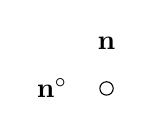
\begin{tikzpicture}[
        dot/.style = {draw, circle, inner sep=0.06cm},
        no/.style = {},
        ]
        \node[no](a) at (0,0) [label=left:$\textbf{n}^\circ$] {};
        \node[no](c) at (0.25, 0.25) [label=above:$\textbf{n}$] {};
        \node[dot](d0) at (0.25,0) [] {};
        \end{tikzpicture}
    \end{figure}
    \begin{itemize}
        \item We can label the node either with a $+$ or a $-$ sign, the choice being
            irrelevant
        \item $H = \mathbb{C}^n \otimes \mathbb{C}^{n\circ} \simeq
            M_n(\mathbb{C})$
        \item $\gamma$ trivial grading ($+1$)
        \item $J$ is a combination of complex conjugation and the flip
            $n\otimes n^\circ$ ($\Rightarrow M_n(\mathbb{C})$ as matrix adjoint)
        \item Because node label is $\pm$ there is no non-zero Dirac operator
        \item $\Rightarrow (A = M_n(\mathbb{C}), H=M_n(\mathbb{C}) , D=0; J=(\cdot)^*,
            \gamma = 1)$
    \end{itemize}
\end{example}
\section{Real Algebras and Krajewski Diagrams}

\begin{definition}
    A real Algebra is a Vector space $A$ over $\mathbb{R}$ with $A\times A
    \rightarrow A$, $(a, b) \mapsto ab$ and $1a = a1 = a \;\; \forall a\in A$
\end{definition}

A real *-algebra is a real algebra with a bilinear map $*:A \rightarrow A$
such that $(ab)^* = b^*a^*$ and $(a^*)^* \;\;\; \forall a,b\in A$
\begin{example}
    Real *-algebra of quaternions $\mathbb{H}$ subalgebra of $M_2(\mathbb{C})$.
    \begin{align}
        \mathbb{H} = \{ \begin{pmatrix}\alpha & \beta \\ -\bar{\beta} &
        \bar{\alpha}\end{pmatrix} : \alpha, \beta \in
            \mathbb{C}\}
    \end{align}
    $\mathbb{H}$ consists of matrices that commute in $M_2(\mathbb{C})$ with
    the operator $I$ defined by:
    \begin{align}
        I\begin{pmatrix}v_1 \\ v_2\end{pmatrix} = \begin{pmatrix}-\bar{v}_2 \\
    \bar{v}_1\end{pmatrix}
    \end{align}
    The involution is the hermitian conjugation of $M_2(\mathbb{C})$.
\end{example}
\begin{MyExercise}
    \textbf{
        \begin{enumerate}
            \item Show that $\mathbb{H}$ is a real *-algebra which contains a
                real subalgebra isomorphic to $\mathbb{C}$.
            \item Show that $\mathbb{H} \otimes_\mathbb{R} \mathbb{C} \simeq
                M_2(\mathbb{C})$ as complex *-algebras.
            \item Show that $M_k(\mathbb{H})$ is areal *-algebra for any $k$
            \item Show that $M_k(\mathbb{H} \otimes_{\mathbb{R}} \mathbb{C}
                \simeq M_{2k}(\mathbb{C})$ as complex *algebras.
        \end{enumerate}
    }
\end{MyExercise}
\begin{definition}
    A representation of a finite-dimensional real * algebra $A$ is a pair $(\pi
    , H$), $H$- Hilbertspace, $\pi : A \rightarrow L(H)$
\end{definition}
\begin{MyExercise}
    Show that there is a one-to-one correspondence between Hilbertspace
    representations of real *-algebras $A$ and complex representations of its
    complexification $A\otimes _\mathbb{R} \mathbb{C}$. Conclude that the
    unique irreducible Hilbertspace representation of $M_k(\mathbb{H})$ is
    $\mathbb{C}^{2k}$
\end{MyExercise}
\begin{lemma}
    Real *-algebra $A$ represented faithfully on a finite dimensional
    Hilbertspace $H$  through a real linear *-algebra map $\pi: A \rightarrow
    L(H)$ hen $A$ is a matrix algebra.
    \begin{align}
        A \simeq \bigoplus _{i=1}^N M_{n_i} (\mathbb{F}_i)
    \end{align}
    Where $\mathbb{F}_i = \mathbb{R}, \mathbb{C}, \mathbb{H}$ depending on $i$.
\end{lemma}
\begin{proof}
    $\pi$ allows $A$ to be considered as a real *-subalgebra of
    $M_{dim(H)}(\mathbb{C}) \Rightarrow A+iA$ complex *-subalgebra of
    $M_{dim(H)}(\mathbb{C})$. Then $A+iA$ is a matrix algebra and $A+iA =
    M_k(\mathbb{C})$ for $k \geq 1$. Thus we have
    \begin{align}
        A \cap iA =
        \begin{cases}
            \{0\} \;\;\;\; \text{if $A = M_k(\mathbb{C})$}\\
            A+iA = M_k(\mathbb{C})
        \end{cases}
    \end{align}
    Furthermore $A$ is a fixed point algebra of an anti-linear automorphism
    $\alpha$ of $M_k(\mathbb{C})$ with $\alpha(a+ib) = a-ib$ for $a, b \in A$.
    Implement $\alpha$ by an anti-linear isometry $I$ on $\mathbb{C}^n$ such
    that $\alpha (x) = I\times I^{-1}\;\;\;\ \forall x\in M_k(\mathbb{C})$.
    Now since $\alpha^2 = 1$, $I^2$ commutes with $M_k(\mathbb{C})$ and is
    proportional to a complex scalar $I^2 = \pm 1 $ and A is the commutant of
    $I$
    \begin{itemize}
        \item if $I^2 = 1 \;\;\ \Rightarrow \;\; \exists \;\;\ \{e_i\}$ ONB of
            $\mathbb{C}^k$ with $Ie_i = e_i$, then $A=M_k(\mathbb{R})$
        \item if $I^2 = -1 \;\;\ \Rightarrow \;\; \exists \;\;\ \{e_i,f_i\}$ ONB of
            $\mathbb{C}^k$ with $Ie_i = f_i$, ($k$ even)\\
            Therefor $I$ must be a $k/2 \times k/2$ matrix because of commutation with
            $M_k(\mathbb{C})$, then $A = M_{k/2} (\mathbb{H})$
    \end{itemize}
\end{proof}
The Krajewski diagrams can also classify real algebras, as long as we take
$\mathbb{F}_i$ for each $i$ into account. That is we enhance the set $\Lambda$
to be
\begin{align}
    \Lambda = \{ \textbf{n}_1 \mathbb{F}_1,\dots, \textbf{n}_N \mathbb{F}_N\}
\end{align}
Reducing in to the previous $\Lambda$ if all $\mathbb{F}_i = \mathbb{C}$.
\section{Classification of Irreducible Geometries}
Classify irreducible real spectral triples based on $M_N(\mathbb{C} \oplus
M_N(\mathbb{C})$ for some $N$
\begin{definition}
    A finite real spectral triple $(A, H, D; J, \gamma)$ is called irreducible
    if the triple $(A, H, J)$ is irreducible, that is when
    \begin{enumerate}
        \item The representation of $A$ and $J$ on $H$ are irreducible
        \item The action of $A$ on $H$ has a separating vector
    \end{enumerate}
\end{definition}

\begin{theorem}
    Let $(A, H, D; J, \gamma)$ be an irreducible finite real spectral triple of
    KO-dimension 6. Then exists a positive integer $N$ such that $A \simeq
    M_N(\mathbb{C}) \oplus M_N(\mathbb{C})$.
\end{theorem}
\begin{proof}
    Let $(A, H, D; J, \gamma)$ be an arbitrary finite real spectral triple,
    corresponding to
    \begin{align}
        &A = \bigoplus_i^{N} M_{n_i}(\mathbb{C})\\
        &H = \bigoplus_{i,j=1}^N \mathbb{C}^{n_i} \otimes
        \mathbb{C}^{n_j\circ} \otimes V_{ij}
    \end{align}
    Remember that each $\mathbb{C}^{n_i} \otimes \mathbb{C}^{n_j}$ is a
    irreducible representation of $A$. In order for $H$ to support the real
    structure $J$ we need both $\mathbb{C}^{n_i} \otimes \mathbb{C}^{n_j}$
    and $\mathbb{C}^{n_j} \otimes \mathbb{C}^{n_i}$. With Lemma \ref{lemma}
    with $J^2 = 1$ with multiplicity $dim(V_{ij}) = 1$ we have such a
    structure. Hence
    \begin{align}
        H = \mathbb{C}^{n_i} \otimes \mathbb{C}^{n_j} \oplus \mathbb{C}^{n_j}
        \otimes \mathbb{C}^{n_i}
    \end{align}
    For $i,j \in \{1, \dots, N\}$
    \newline

    For the second condition (existence of the separating vector). The
    representations of $A$ in $H$ are only faithful if $A = M_{n_i}(\mathbb{C})
    \oplus M_{n_j}(\mathbb{C})$. The stronger condition applies $n_i = n_j$
    then we have $A' \xi = H$ with the commutant of $A$ and $\xi \in H$ the
    separating vector. Normally since $A' = M_{n_j}(\mathbb{C}) \oplus
    M_{n_i}(\mathbb{C})$ with $dim(A') = n_i^2 + n_j^2$ and $dim(H) = 2n_i n_j$
    we have a equality $n_i = n_j$.
\end{proof}
\end{document}





